\documentclass{segabs}
\usepackage{xspace,color,amsmath}
\usepackage{amssymb}
\usepackage{hyperref}

% Handy commands
\renewcommand{\thefootnote}{\fnsymbol{footnote}}
\newcommand{\SimPEG}{\textsc{SimPEG}\xspace}
\newcommand{\simpegEM}{\textsc{simpegEM}\xspace}
\newcommand{\TODO}[1]{{\color{red} TODO: #1}}

% Math
\newcommand{\curl}{{\nabla \times}}
\renewcommand{\div}{{\nabla \cdot}}
\newcommand{\meshP}{\emph{mesh}$^p$\xspace}
\newcommand{\meshS}{\emph{mesh}$^s$\xspace}

\begin{document}

\title{Modelling electromagnetic problems in the presence of cased wells} %add something about different meshes too ?

\author{Lindsey J. Heagy$^1$ \footnotemark[1], Rowan Cockett$^1$, Douglas W. Oldenburg$^1$ and Michael Wilt$^2$ \\ $^1$University of British Columbia: Geophysical Inversion Facility, $^2$GroundMetrics}
\email{lheagy@eos.ubc.ca}

% \footer{Example}
% \lefthead{Heagy, Cockett, Oldenburg \& Wilt}
% \righthead{Modelling EM problems in the presence of cased wells}

\maketitle

\begin{abstract}
	Electrical conductivity can be a diagnostic physical property for distinguishing geologic units and delineating the distribution of fluids such as hydrocarbons and saline water within these units. Electromagnetic (EM) methods are sensitive to conductivity contrasts and can be used to characterize them. They are increasingly being applied in settings where cased wells are present. Most commonly-used casing materials, such as steel, are highly conductive, have a significant, often variable, magnetic permeability, and therefore significantly impact the behavior of the EM fields and fluxes. The aim of this paper is to revisit numerical modelling strategies to investigate the role of various properties and complexities due to the casing, and present a modelling and inversion strategy, using a primary-secondary approach, for capturing the impacts of both the variable casing and three dimensional geologic structures on EM data.
% \vspace{-8pt}
\end{abstract}

% \vspace{-8pt}
\section{Introduction}
% \vspace{-8pt}
Variations in subsurface electrical conductivity have been used as a diagnostic physical property in sedimentary settings for characterizing geologic formations, and the properties and distribution of fluids within those formations. Hydrocarbons and CO$_2$ are much more resistive than saline formation fluids, and are typically more resistive than fluids injected during enhanced recovery projects. This contrast has been the target of cross-well, surface-to-borehole and borehole-to-surface electromagnetic (EM) methods for monitoring and characterization applications (cf. \cite{Marsala2008, Marsala2011, Wilt1995}). These surveys are typically conducted in settings that have cased wells, and the many of the associated modelling strategies have focused on characterizing the distortion of the transmitted and received signals. \cite{cuevas2014} provides analytical solutions for dipolar sources in an infinite cylinder, which has supported modelling and inversion approaches that replace the casing in a model with an ``equivalent source'' created using a series of electric or magnetic dipoles (cf. \cite{cuevas2012}). Alternatively, some approaches to the inverse problem aim to bypass characterizing the response of the casing through constructing a datum that is independent of the casing effect and taking ratios of measured electromagnetic responses \citep{Gao2008, Liu2008}. More recently, there has been growing interest in using the casing as an extended source for carrying signal to reservoir depths \citep{Commer2015, Hoversten2014, Marsala2014, cuevas2014eage}. The aim of this paper is to revisit modelling strategies to allow for the investigation of the role of various properties and complexities due to the casing, and present a modelling and inversion strategy for capturing the impacts of both the variable casing and three dimensional geologic structures on EM data.

Modelling and inverting EM geophysical data collected in settings including cased wells presents several significant challenges. Most wells are cased with carbon steel, which has both a large electrical conductivity ($\sim 5.5\times 10^6$ S/m), and magnetic permeability ($\sim 50 \mu_0$) \citep{wuhabashy1994}. This is a large contrast to typical geologic settings, with conductivities typically less than 1 S/m and permeabilities similar to that of free space, $\mu_0$. As a result, the casing may have a significant impact on the behavior of the EM fields and fluxes. The properties, in particular, magnetic susceptibility, as well as casing thickness can vary along the length of the well, depending both on the quality of the steel and the state of corrosion, adding another level of complexity to the situation. Well logging tools, such as that described by \cite{Brill2012} have been developed to characterize these variations.

Not only does casing introduce a large, variable, physical property contrast, its geometry and scale add to the difficulty. Well casing is cylindrical in shape and only millimeters to centimeters thick, while the geologic structures we aim to characterize with the geophysical survey have three dimensional variations in electrical conductivity on the scale of hundreds of meters to kilometers. Approaches tailored to accurately modelling the impact of the casing may be geometrically incompatible or computationally prohibitive to use when reservoir-scale, three-dimensional geologic structures are included in the conductivity model.

In this paper, we concentrate on two aspects of this problem. The first looks at the details of modelling a casing with complicated physical properties and examining the effects of putting different sources (both galvanic and inductive) at various locations in/on the casing. Second, we demonstrate how a primary-secondary approach for solving Maxwell's equations (cf. \cite{Haber2014a}) may be used to model three-dimensional geologic structures in settings including cased wells. This approach allows the problem of simulating the casing and the three dimensional geologic structures to be treated as two distinct problems. We first compute the response due to the transmitter and casing in a simple geologic background. In particular, we consider a vertical well in a one-dimensional geologic background and exploit cylindrical symmetry for computing the primary response. Secondly, we interpolate these fields to the secondary mesh, where they are used as a source for the secondary response. By decoupling these two problems the mesh design, computational strategies and model complexities for each problem can be treated separately.

% \vspace{-8pt}
\section{Approach}
% \vspace{-8pt}
To motivate our discussion, we consider the model shown in Figure \ref{fig:CasingGeoModel}, consisting of a vertical well in a layered background with a three- dimensional, resistive region in the reservoir layer, which is the target of the geophysical survey. The casing is composed of carbon steel ($5.5 \times 10^6 S/m$) and is filled with water-based drilling mud ($1 S/m$). We will consider three casing models in which we vary the magnetic permeability. In the first, we neglect any contributions of permeability, treating it as equal to that of free space ($\mu_0$); in the second we use a constant value of $50\mu_0$; in the third we consider a casing with variable permeability by including a segment which has a permeability of $150\mu_0$. For brevity of this example, we neglect surface casing and conductivity variations introduced by cement and invasion of drilling fluids into the surrounding formations. We employ a simple geologic background consisting of four layers, as shown in Figure \ref{fig:CasingGeoModel} and consider the frequency domain electromagnetic (FDEM) problem with three sources (illustrated in Figure \ref{fig:CasingGeoModel}) for inputting EM energy into the system: (1) using a downhole magnetic dipole source, (2) using a downhole galvanic source, and (3) exciting the casing at the surface using a galvanic source.
\begin{figure}[h!]
	\centering
	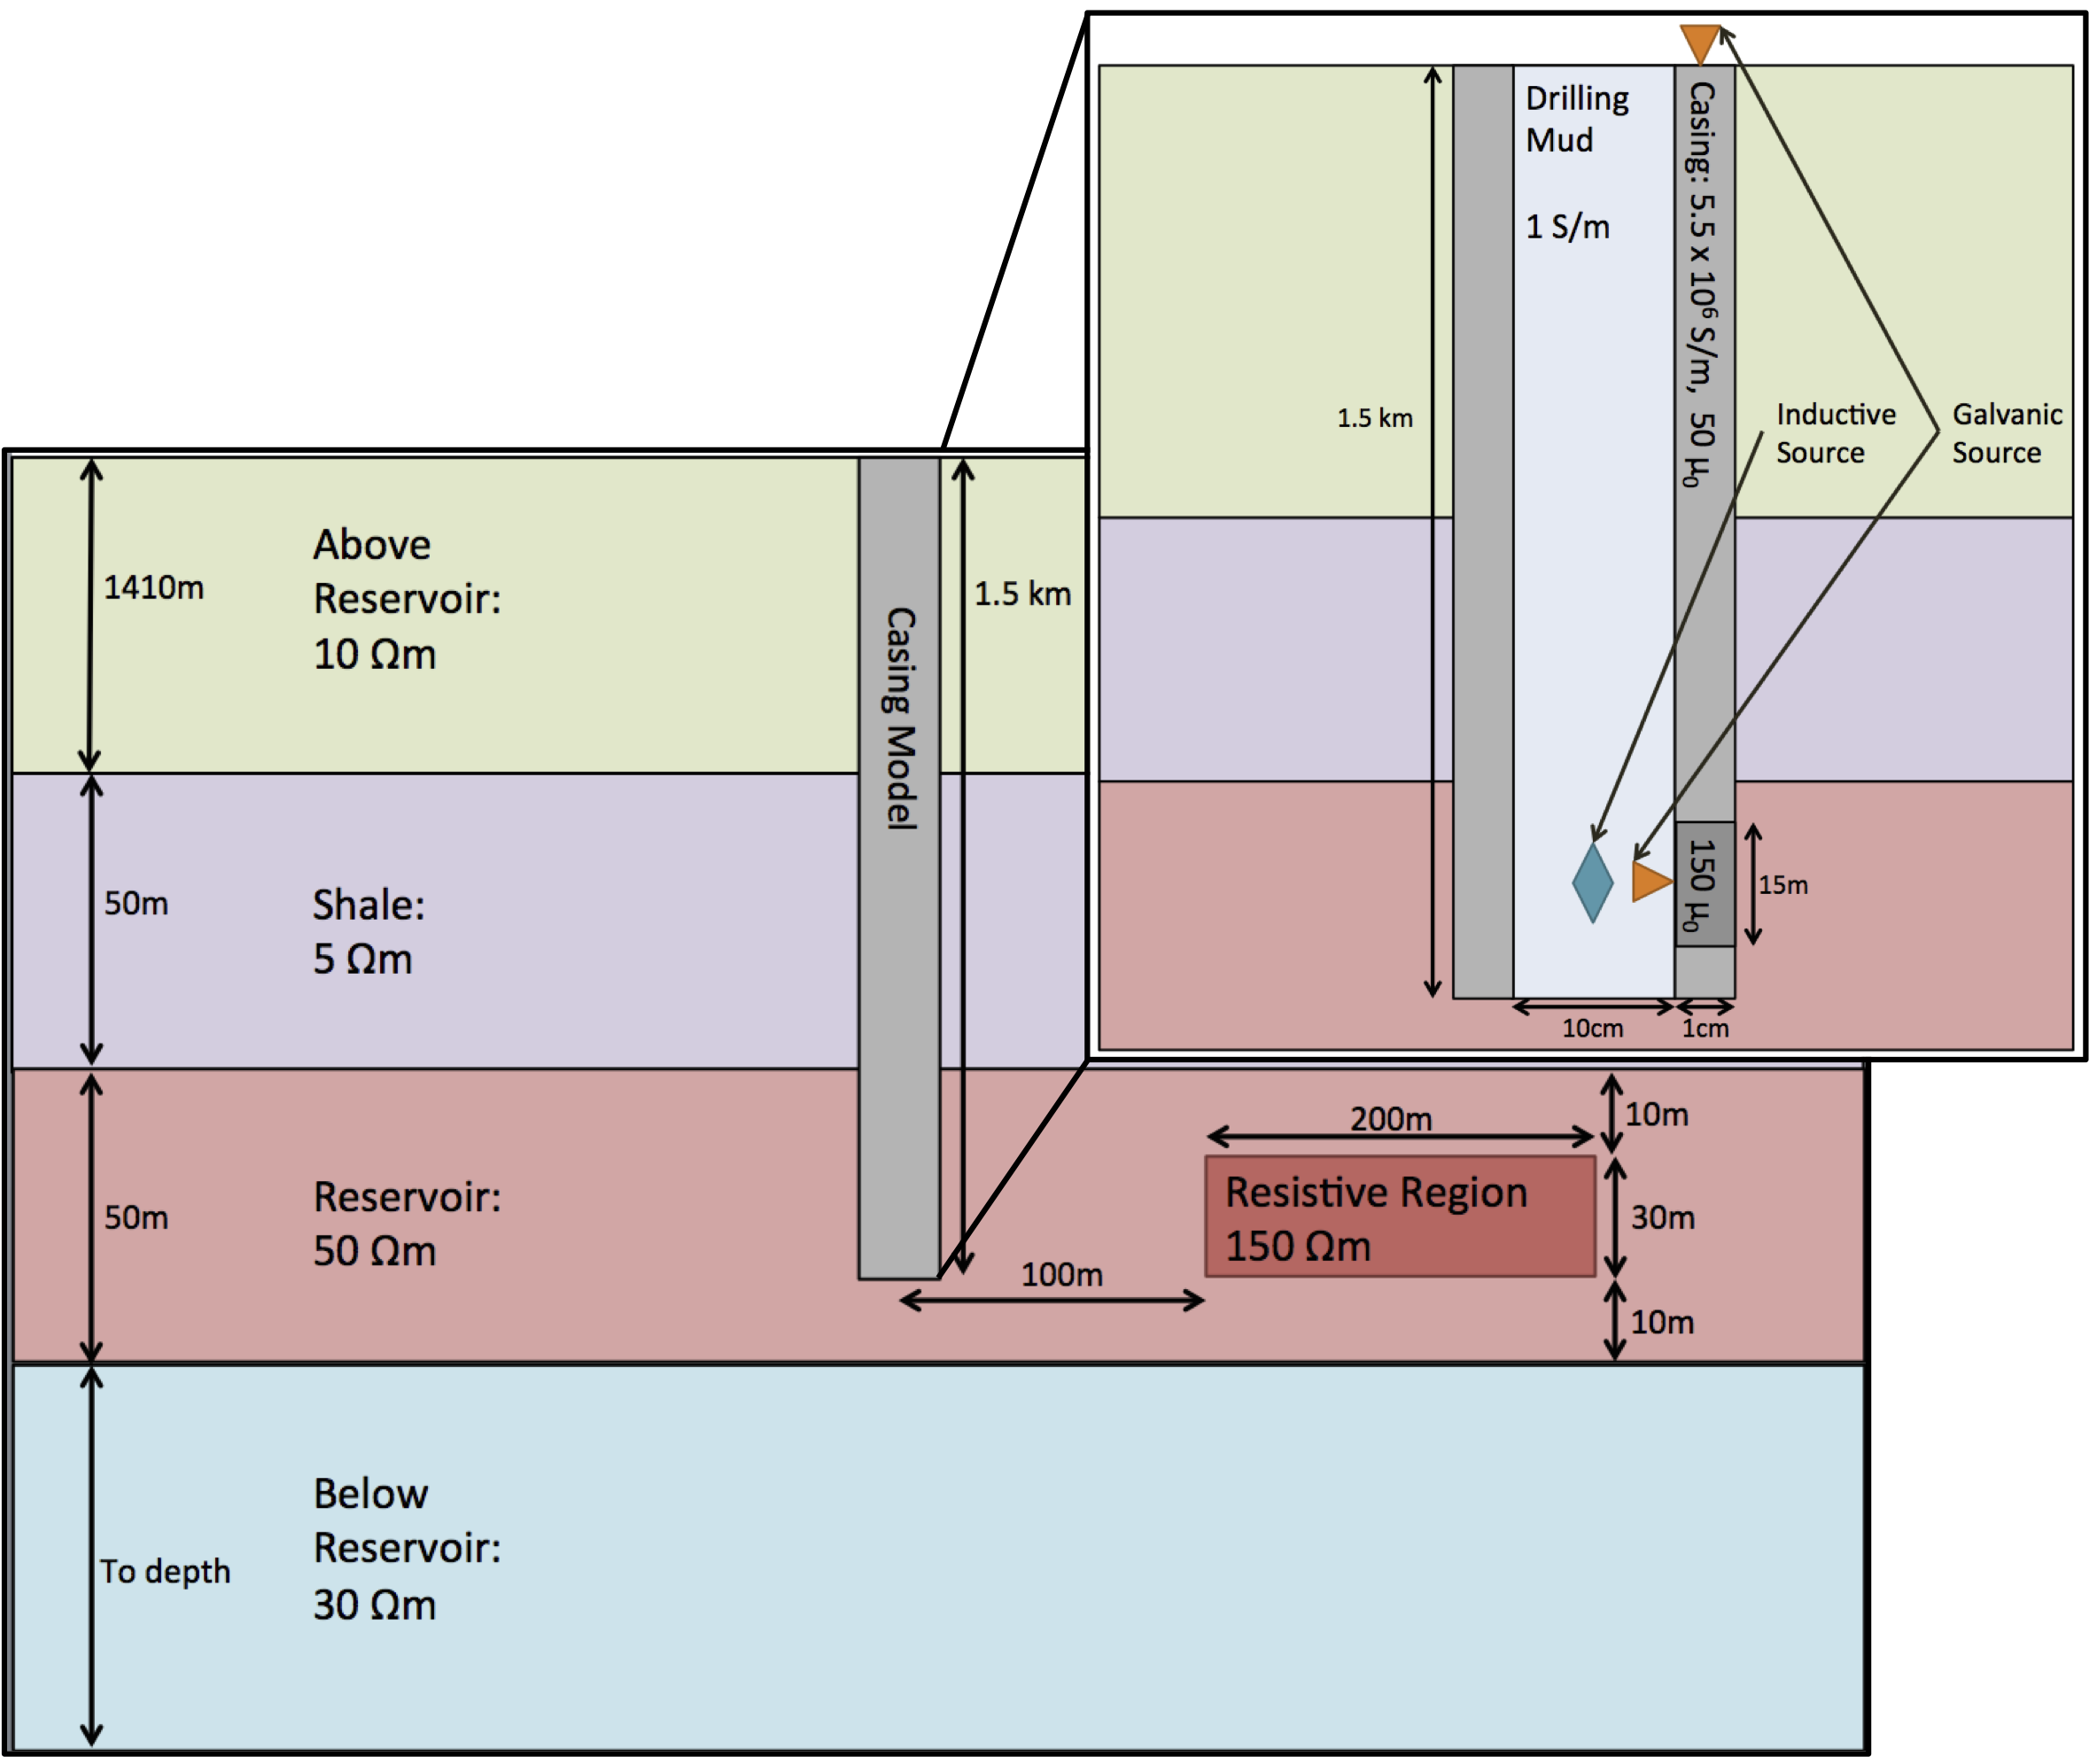
\includegraphics[width=0.9\columnwidth]{./Figures/CasingGeoModel}
	\caption{Sketch of casing and geologic model (not to scale).}
	\label{fig:CasingGeoModel}
\end{figure}

\subsection{Modelling the casing: Primary}
We begin by considering approaches for modelling the casing and associated structures, as shown in the upper right panel of Figure \ref{fig:CasingGeoModel}. The background geologic model is one-dimensional, and for the sources we are considering, the problem is cylindrically symmetric. We take advantage of the symmetry using a 2.5D cylindrical mesh to calculate the primary EM response. To numerically simulate the FDEM problem, we examine two formulations of Maxwell's equations: the E-B and H-J formulations. Each of these formulations is a set of partial differential equations connecting a field and a flux. The E-B formulation links the electric field, $\vec{E}$ and the magnetic flux density $\vec{B}$:
\begin{equation}
	\begin{split}
		\curl \vec{E} + i \omega \vec{B} = 0 \\
		\curl \mu^{-1} \vec{B} - \sigma \vec{E} = \vec{s}
	\end{split}
	\label{eq:maxwellEB}
\end{equation}
where $i$ is the imaginary unit, $\omega = 2\pi f$ is the angular frequency, $\mu$ is the magnetic permeability, $\sigma$ is the electrical conductivity, and $\vec{s}$ is the source current density. Alternatively, we can consider the H-J formulation which uses the magnetic field $\vec{H}$, and the current density $\vec{J}$. This formulation is related to the E-B formulation by the constitutive relations: $\vec{J} = \sigma \vec{E}$, and $\vec{B} = \mu \vec{H}$ and is given by
\begin{equation}
	\begin{split}
		\curl \rho \vec{J} + i \omega \mu \vec{H} = 0 \\
		\curl \vec{H} - \vec{J} = \vec{s}
	\end{split}
	\label{eq:maxwellHJ}
\end{equation}
where $\rho = \sigma^{-1}$ is resistivity. Although equivalent in the continuous form, the act of discretizing makes these two formulations distinct.

To numerically model Maxwell's equations, we use a mimetic finite volume approach with a staggered grid, where fields are discretized on edges, fluxes on faces, and physical properties in cell centers (cf. \cite{Haber2014a}), as shown in Figure~\ref{fig:fvcells} and summarized for the two formulations of Maxwell's equations in Table~\ref{tab:DiscEBHJ}. For the cylindrically symmetric mesh (Figure~\ref{fig:fvcells}b), edges exist only in the $\theta$ direction, while faces exist only in the $r$ and $z$ directions; there are no nodes. The imposed symmetry present in this discretization means that fields are restricted to having only a $\theta$ component, while fluxes only have vertical and radial components. These distinctions are important when considering the differences between inductive and galvanic sources. For inductive sources, we require a modelling strategy that allows magnetic flux to have vertical and radial components. For inductive sources, however, we require that the current density has vertical and radial components. To achieve these modelling requirements, we use the E-B formulation for inductive sources, and the H-J formulation for galvanic sources, as summarized in Table~\ref{tab:DiscEBHJ} and Figure~\ref{fig:fvcells}.
\begin{figure}[h!]
	\centering
	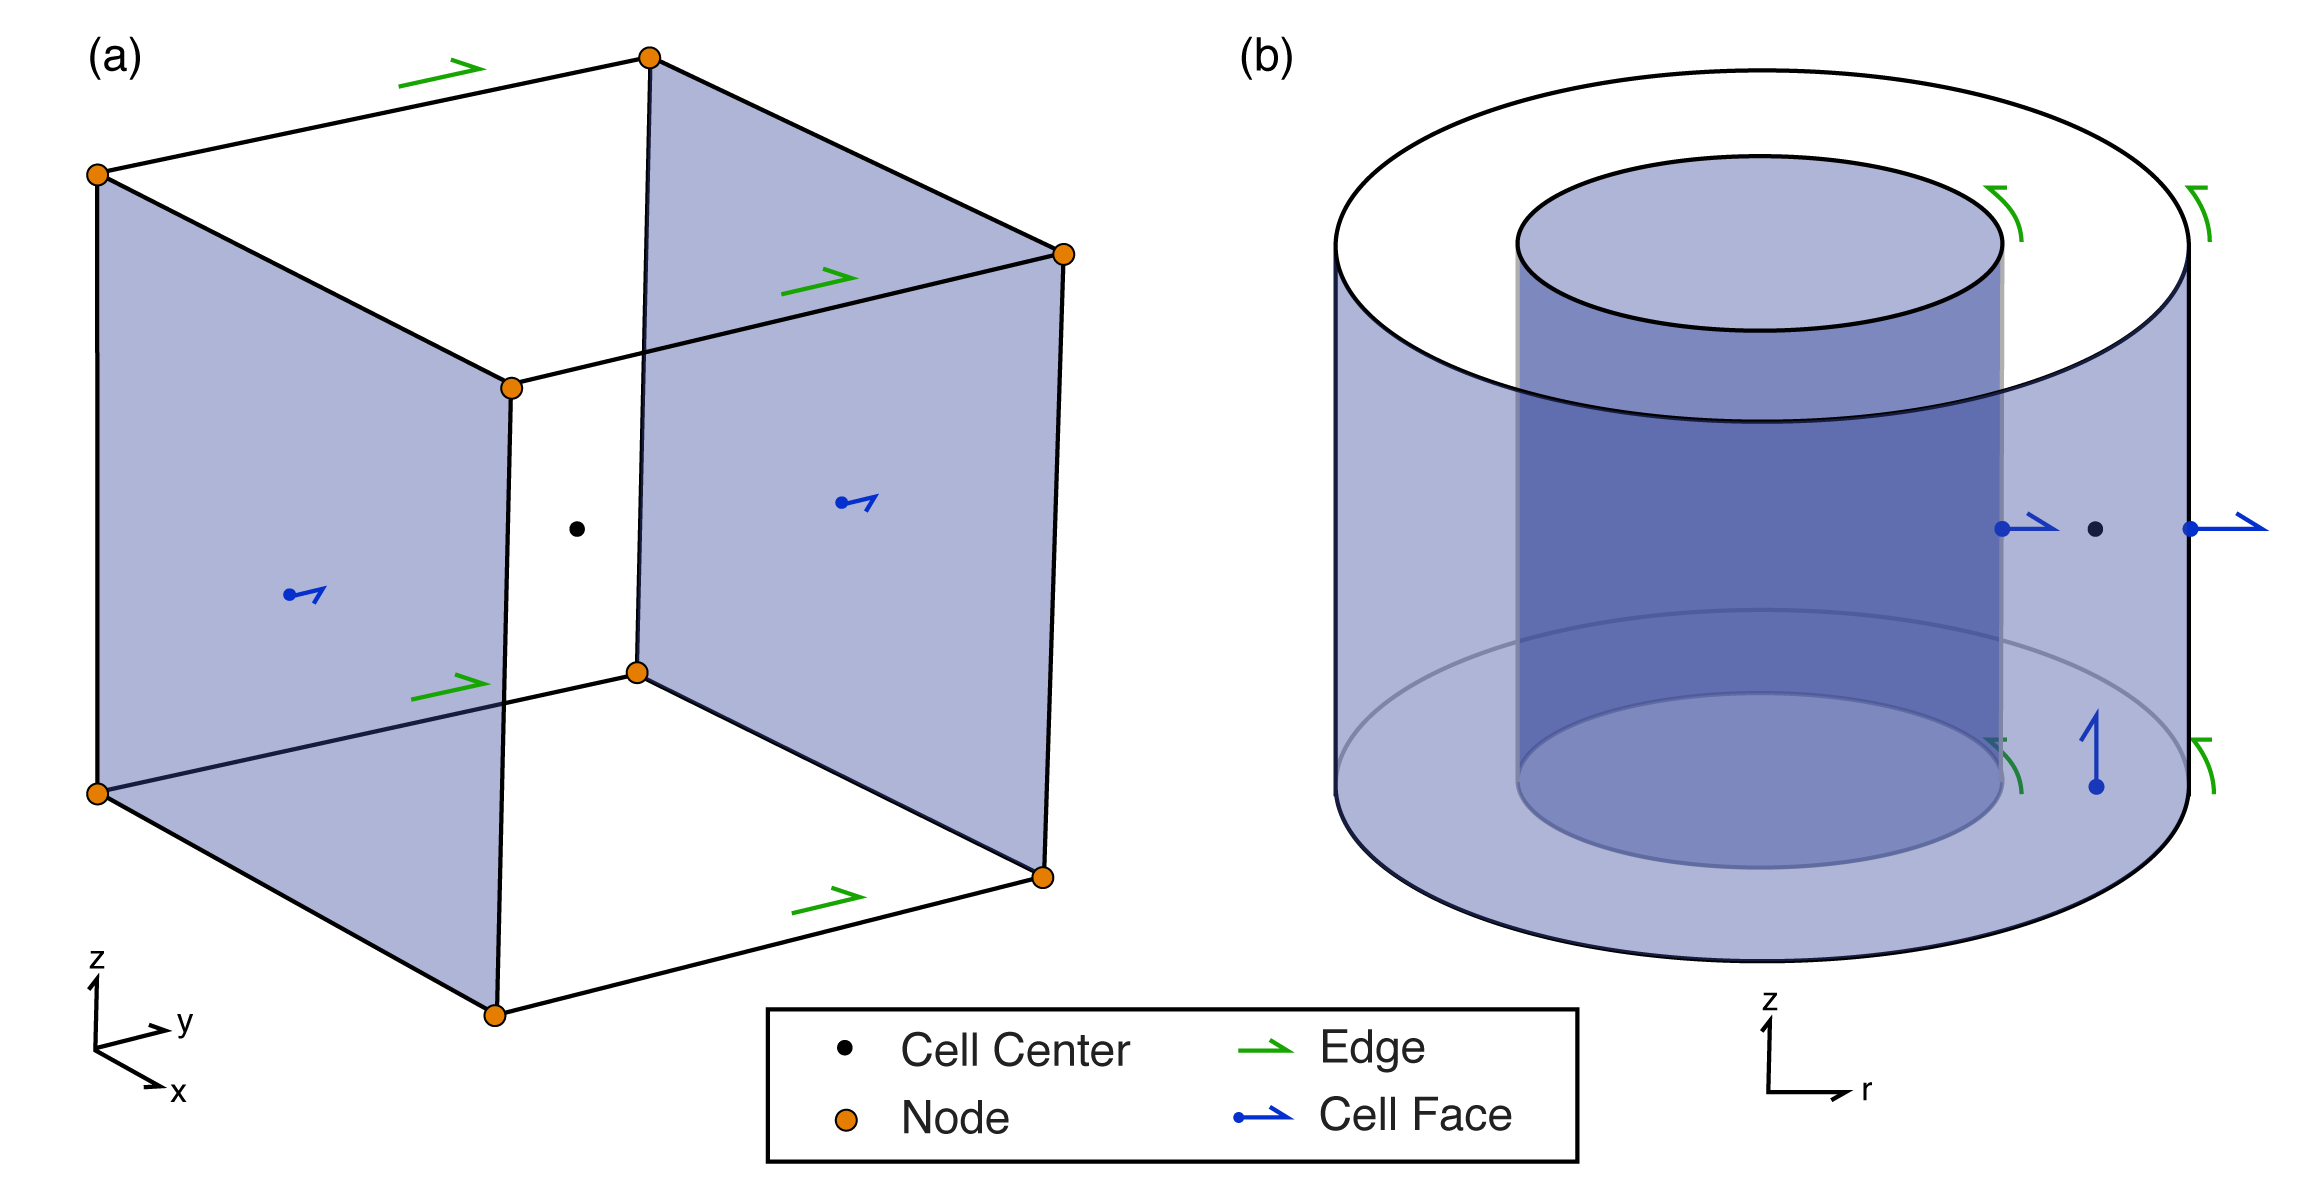
\includegraphics[width=0.9\columnwidth]{./Figures/FVcubes}
	\caption{A finite volume mesh cell showing locations of scalar and vector properties in (a) cartesian coordinates and (b) cylindrical coordinates.}
	\label{fig:fvcells}
\end{figure}
\begin{table}[h!]
\centering
\begin{tabular}{| l | l | l | l |}
	\hline
	\textbf{Formulation} & \textbf{cell centers} & \textbf{edges} & \textbf{faces} \\
	\hline
	E-B                  & $\mu^{-1}$, $\sigma$  & $\vec{E}$      & $\vec{B}$      \\
	H-J                  & $\mu$, $\rho$              & $\vec{H}$      & $\vec{J}$       \\
	\hline
	\end{tabular}
	\label{tab:DiscEBHJ}
	\caption{Discretization of variables for two formulations of the FDEM problem.}
\end{table}
\subsubsection{Example}
Returning to the casing model shown in the top right hand side of Figure~\ref{fig:CasingGeoModel}, we forward-simulated the EM response of the well casing and 1D geologic background for three sources: (1) a downhole magnetic source, (2) a downhole galvanic source, and (3) a surface galvanic source. For the following simulations we use \SimPEG and \simpegEM \citep{SimPEG, SimPEGEM}.

In Figure~\ref{fig:varyFreq}, we compare the in-phase, horizontal component of: (a) the magnetic flux resulting from excitation with the downhole inductive source; (b) the current density from the downhole galvanic source; and (c) the current density from the surface galvanic source at a distance of 100m from the center of the well. We show the in-phase responses for two casing models: (1) where the permeability of the casing is assumed to be that of free space (solid lines), and (2) where the permeability of the casing is a constant value of $50 \mu_0$ along the well (dashed lines). Each of these two scenarios is completed for frequencies of 0.1 Hz (blue), 1 Hz (green) and 5 Hz (red). For these comparisons, we are interested in the relative responses in each scenario, irrespective of the source strength, as such, note that the responses have been normalized. For both the downhole magnetic and galvanic sources, the impact of $\mu$ on the signal is minimal until the frequency is high enough for inductive effects to be observed, as seen by the 5Hz responses for both of these sources. For the surface galvanic source, the impact of the variations in $\mu$ is apparent over a larger range of frequencies, as we can see differences in both the 0.1Hz and 5Hz signals. The difference between the 5Hz signals for the two casing models is more significant for the surface galvanic source (c) then the downhole sources, (a) and (b), as may be expected, due to the larger distance over which the signal has travelled in the casing.
\begin{figure}[h!]
	\centering
	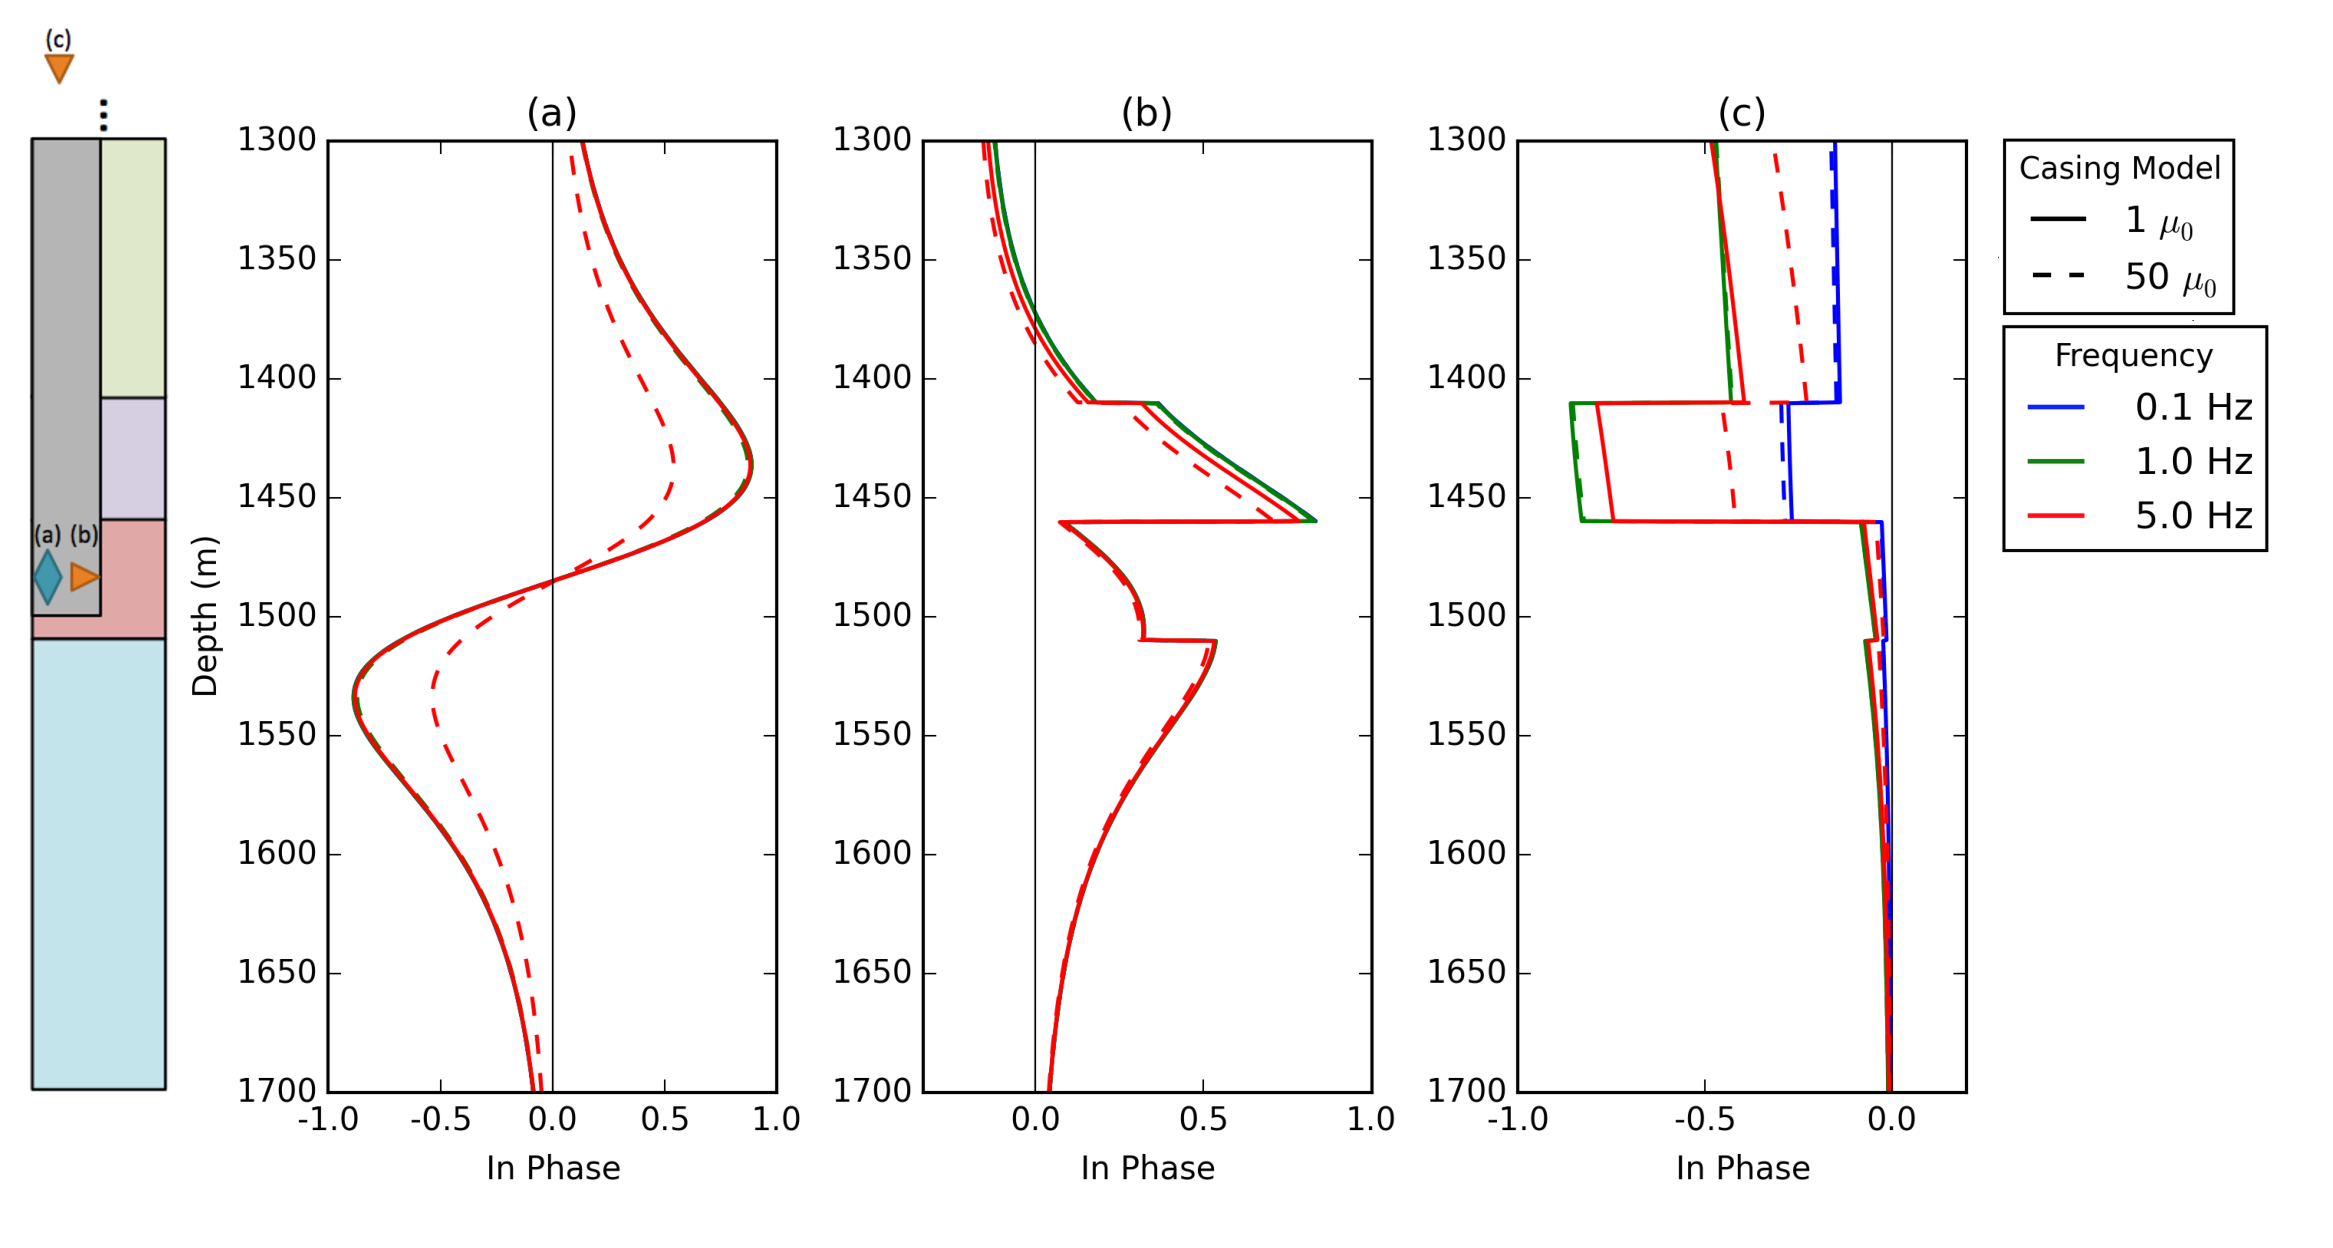
\includegraphics[width=1\columnwidth]{./Figures/VaryFreq}
	\caption{Normalized in-phase responses. Horizontal component of:  (a) magnetic flux from the magnetic dipole source, (b) current density for the downhole galvanic source, (c) current density for the surface galvanic source at a radial distance of 100m from the center of the well for frequencies of 0.1Hz (blue), 1Hz (green)  and 5Hz (red). The solid lines treat the permeability of the casing as equal to $\mu_0$, and the dashed lines use a permeability of $50 \mu_0$. }
	\label{fig:varyFreq}
\end{figure}
To examine the impact of variable magnetic permeability on the behavior of the fields, we now include a 15 m segment having a permeability of $150 \mu_0$ in our casing model, as shown in the illustration in Figure~\ref{fig:CasingGeoModel}. In Figure~\ref{fig:AnomMu}, we show the normalized, in-phase horizontal component of (a) the magnetic flux for the downhole inductive source, (b) the current density for the downhole galvanic source, and (c) the current density for the surface galvanic source, all at a distance of 100m from the center of the well. The solid lines are the casing models with $\mu = \mu_0$, the dashed is the casing model with a constant value of $\mu = 50 \mu_0$ and the dotted lines are the model with the segment of highly permeable material ($150 \mu_0$). For the downhole magnetic source, we see that the highly permeable segment has a significant impact as frequency is increased. These effects are similarly observed for the downhole galvanic source, but their role is less pronounced. For the surface galvanic source, we see that including a highly permeable section at depth has minimal impact beyond that observed for the scenario where $\mu = 50\mu_0$.
\begin{figure}[h!]
	\centering
	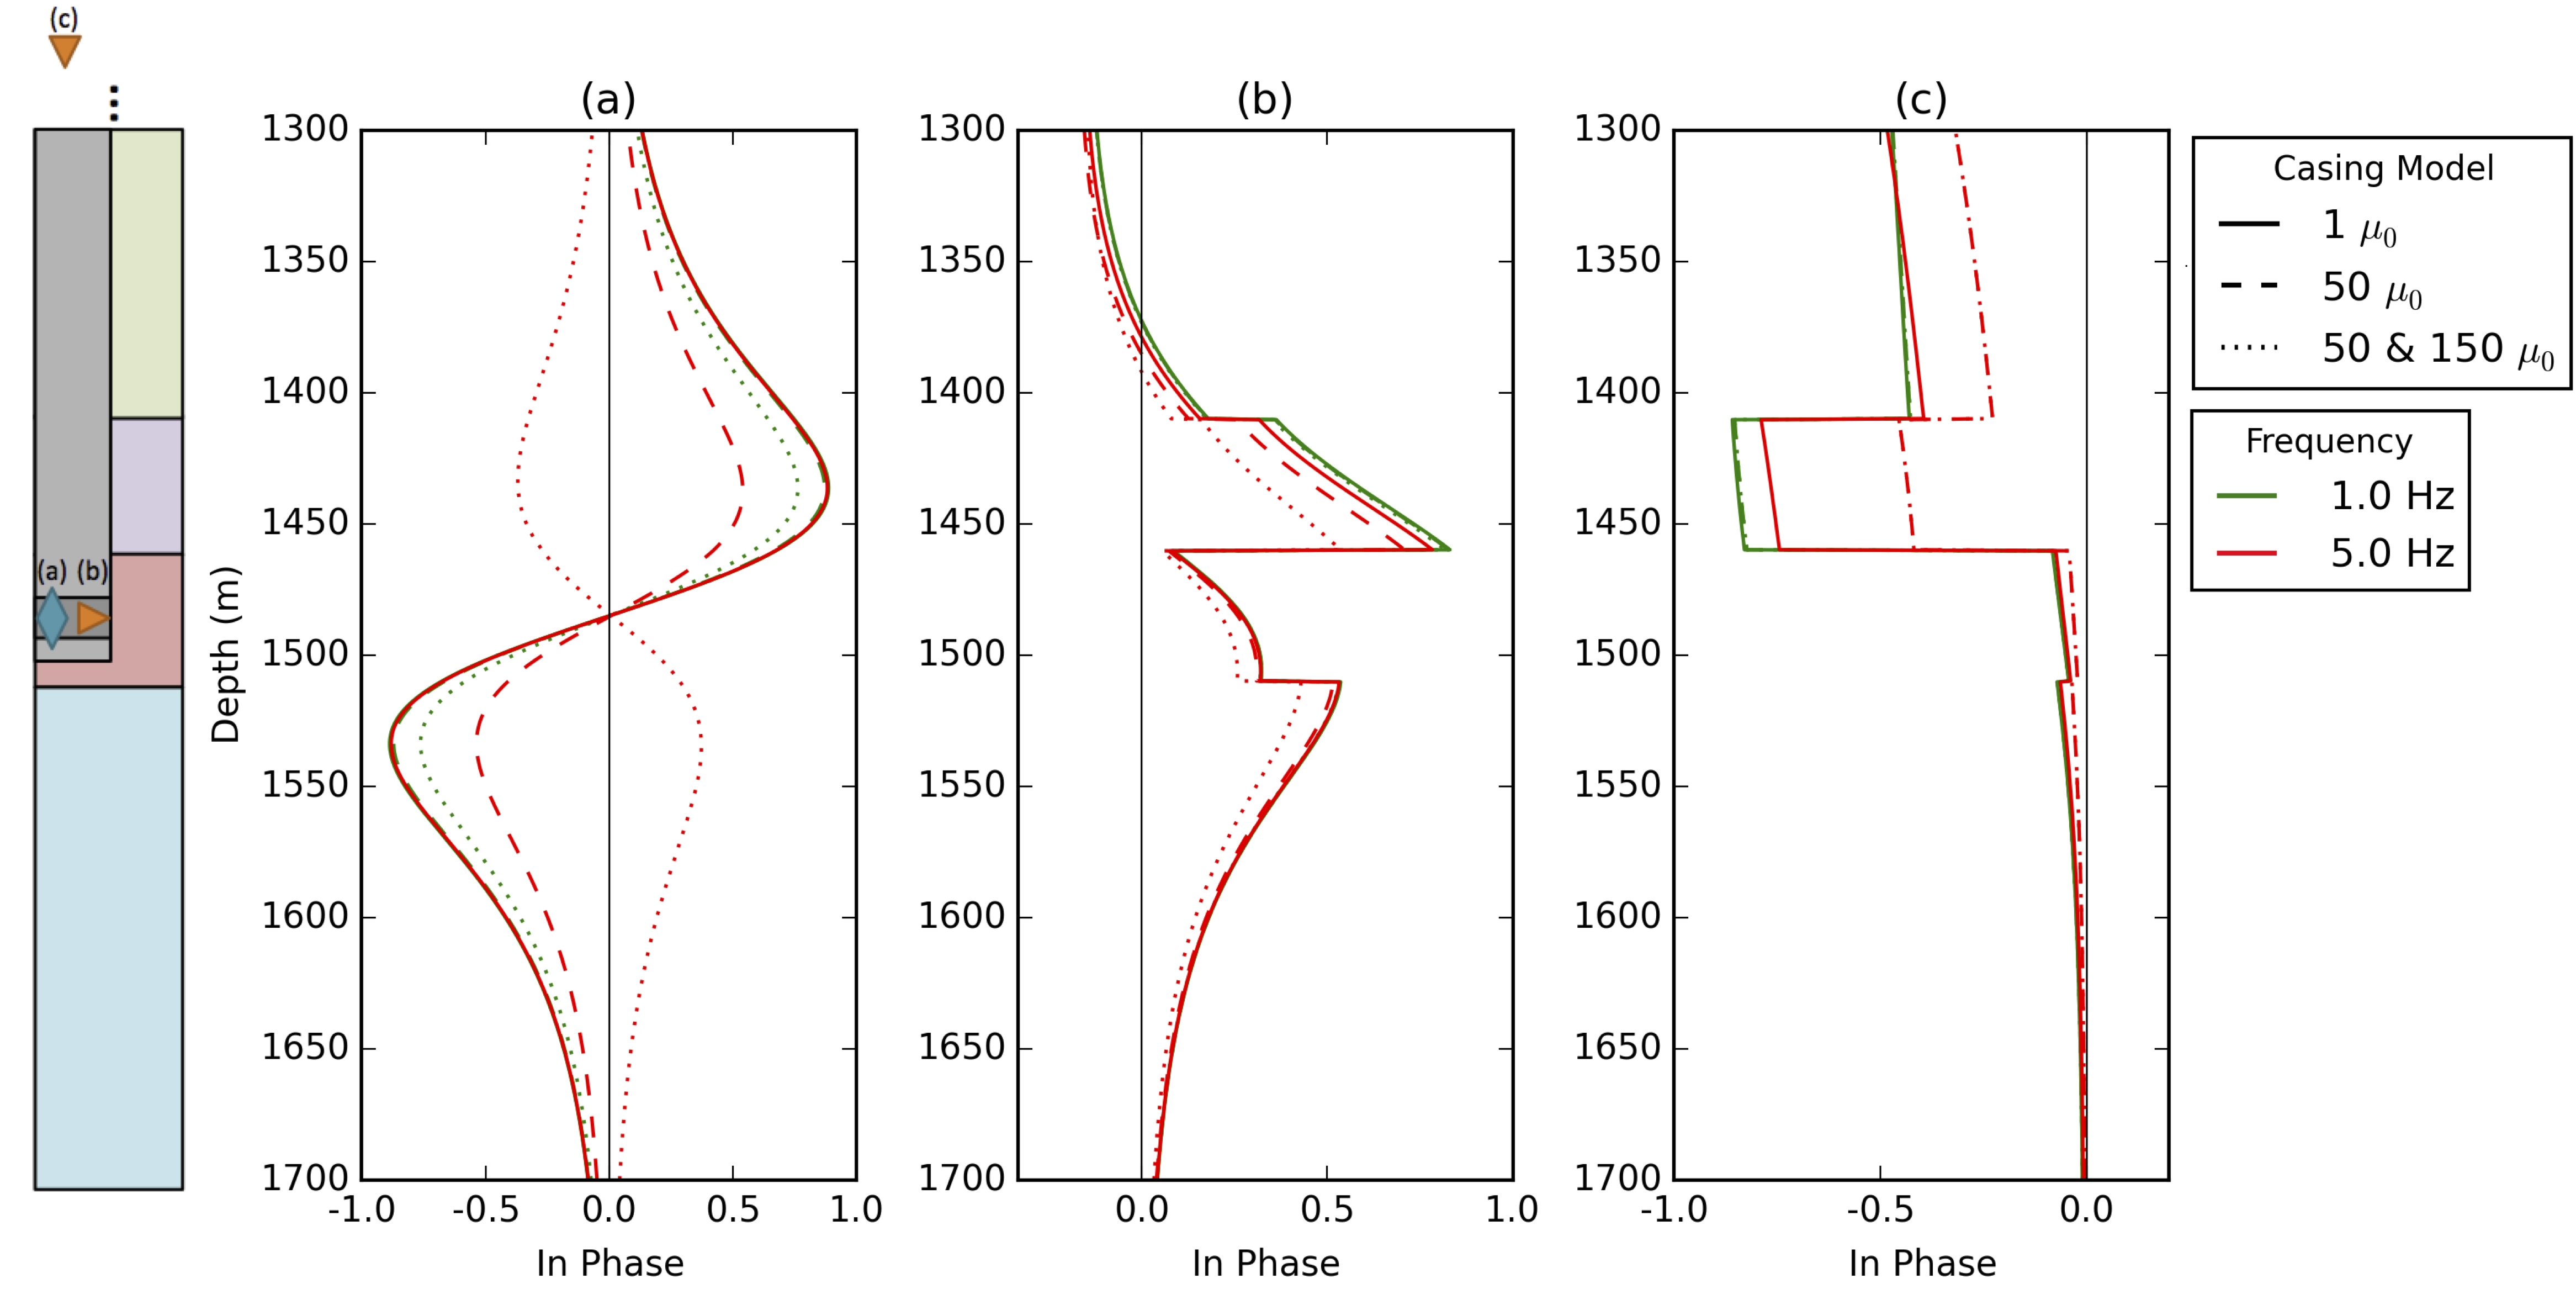
\includegraphics[width=1\columnwidth]{./Figures/AnomMu}
	\caption{Normalized in-phase response. Horizontal component of the (a) magnetic flux from the magnetic dipole source, (b) current density for the downhole galvanic source, (c) current density for the surface galvanic source at a radial distance of 100m from the center of the well for frequencies of 1Hz (green) and 5Hz (red). The solid lines treat the permeability of the casing as equal to $\mu_0$, the dashed lines use a permeability of $50 \mu_0$, and the dotted lines are the model having a 15 m segment of casing with a permeability of $150 \mu_0$.}
	\label{fig:AnomMu}
\end{figure}
Even for the simple casing model we have considered, we see that the impact of the casing's magnetic permeability on the signal can be significant depending on the source type, location, and frequency. By first considering a simple geologic background, we have focused our modelling efforts on understanding the impact of parameters and structures associated with the casing. Further complexities associated with the casing, such as surface casing, cement, drilling fluid invasion into the surrounding formations, and variations in casing thickness may also be incorporated at this stage in the primary-secondary approach to the modelling.

\subsection{Primary-Secondary}
Next, we need a means of linking the two problems: modelling the casing, and modelling the three dimensional geologic structures. For this, we consider the primary-secondary approach. We will develop this using the E-B formulation of Maxwell's equations (\ref{eq:maxwellEB}), but the same procedure can be followed in either formulation. We consider the physical properties, fields, and fluxes to be composed of two components, a primary and a secondary: $\sigma = \sigma_p + \sigma_s$, $\mu^{-1} = \mu_p^{-1} + \mu_s^{-1}$, $\vec{E} = \vec{E}_p + \vec{E}_s$ and $\vec{B} = \vec{B}_p + \vec{B}_s$. We choose the primary physical properties to capture the physical properties of the casing and simple geologic background, as discussed in the previous section and satisfies
\begin{equation}
\begin{split}
	\curl \vec{E}_p + i \omega \vec{B}_p = 0 \\
	\curl \mu^{-1}_p \vec{B}_p - \sigma_p \vec{E}_p = \vec{s}
\end{split}
\label{eq:primary}
\end{equation}
The secondary fields then must satisfy
\begin{equation}
\begin{split}
	\curl \vec{E}_s + i \omega \vec{B}_s = 0 \\
	\curl \mu^{-1}\vec{B}_s - \sigma \vec{E}_s = \vec{q} \\
	\vec{q} =  - (\curl (\mu^{-1} - \mu_p^{-1} ) \vec{B}_p - (\sigma - \sigma_p) \vec{E}_p)
\end{split}
\label{eq:secondary}
\end{equation}
That is, we have defined the source term: $\vec{q}$ for the secondary fields. This source is located where there are differences between the full physical property models of $\mu^{-1}$ and $\sigma$ and the physical property models captured by the primary, $mu^{-1}_p$ and $\sigma_p$. In the case of the model shown in Figure~\ref{fig:CasingGeoModel}, this is the resistive region of the reservoir.  As this region has $\mu = \mu_0$, it is only the contrast in electrical conductivity that contributes to the source term for the secondary, namely our new source is $\vec{q} = (\sigma - \sigma_p) \vec{E}_p$.

To simulate the secondary fields, we want to use a mesh that is suited for capturing large, three-dimensional structures. In this case, we use a Cartesian-coordinate tensor mesh. To link the two problems, the first, on a cylindrical mesh and the second on a Cartesian mesh, we require an interpolation strategy for the fields and fluxes. By construction, the fields and fluxes are defined on the mesh so that they are continuous and smoothly varying, so the interpolation is straightforward. In order to maintain that our fluxes are divergence free over the domain ($\div \vec{B} = 0$ in the E-B formulation, and $\div \vec{J} = 0$ in the H-J formulation), we interpolate the field (E or H) and compute the associated flux (B or J) through a discrete curl operation on the secondary mesh. The mimetic properties of the discretization ensure that the discrete curl is in the null space of the discrete divergence, so the fluxes will be divergence free on the secondary mesh. With the primary fields and fluxes defined on this mesh, the new source term is then computed and is used to calculate the secondary fields and fluxes. In Figure~\ref{fig:secondarySource}, we show a depth slice of the the source term, as described in equation \ref{eq:secondary} for the magnetic dipole source at 1 Hz, with the casing model having with a constant magnetic permeability of $50 \mu_0$. The source term is localized to the 200m $\times$ 200m resistive region in Figure \ref{fig:CasingGeoModel} which was not included in the primary conductivity model (equation \ref{eq:secondary}).
\begin{figure}[h!]
	\centering
	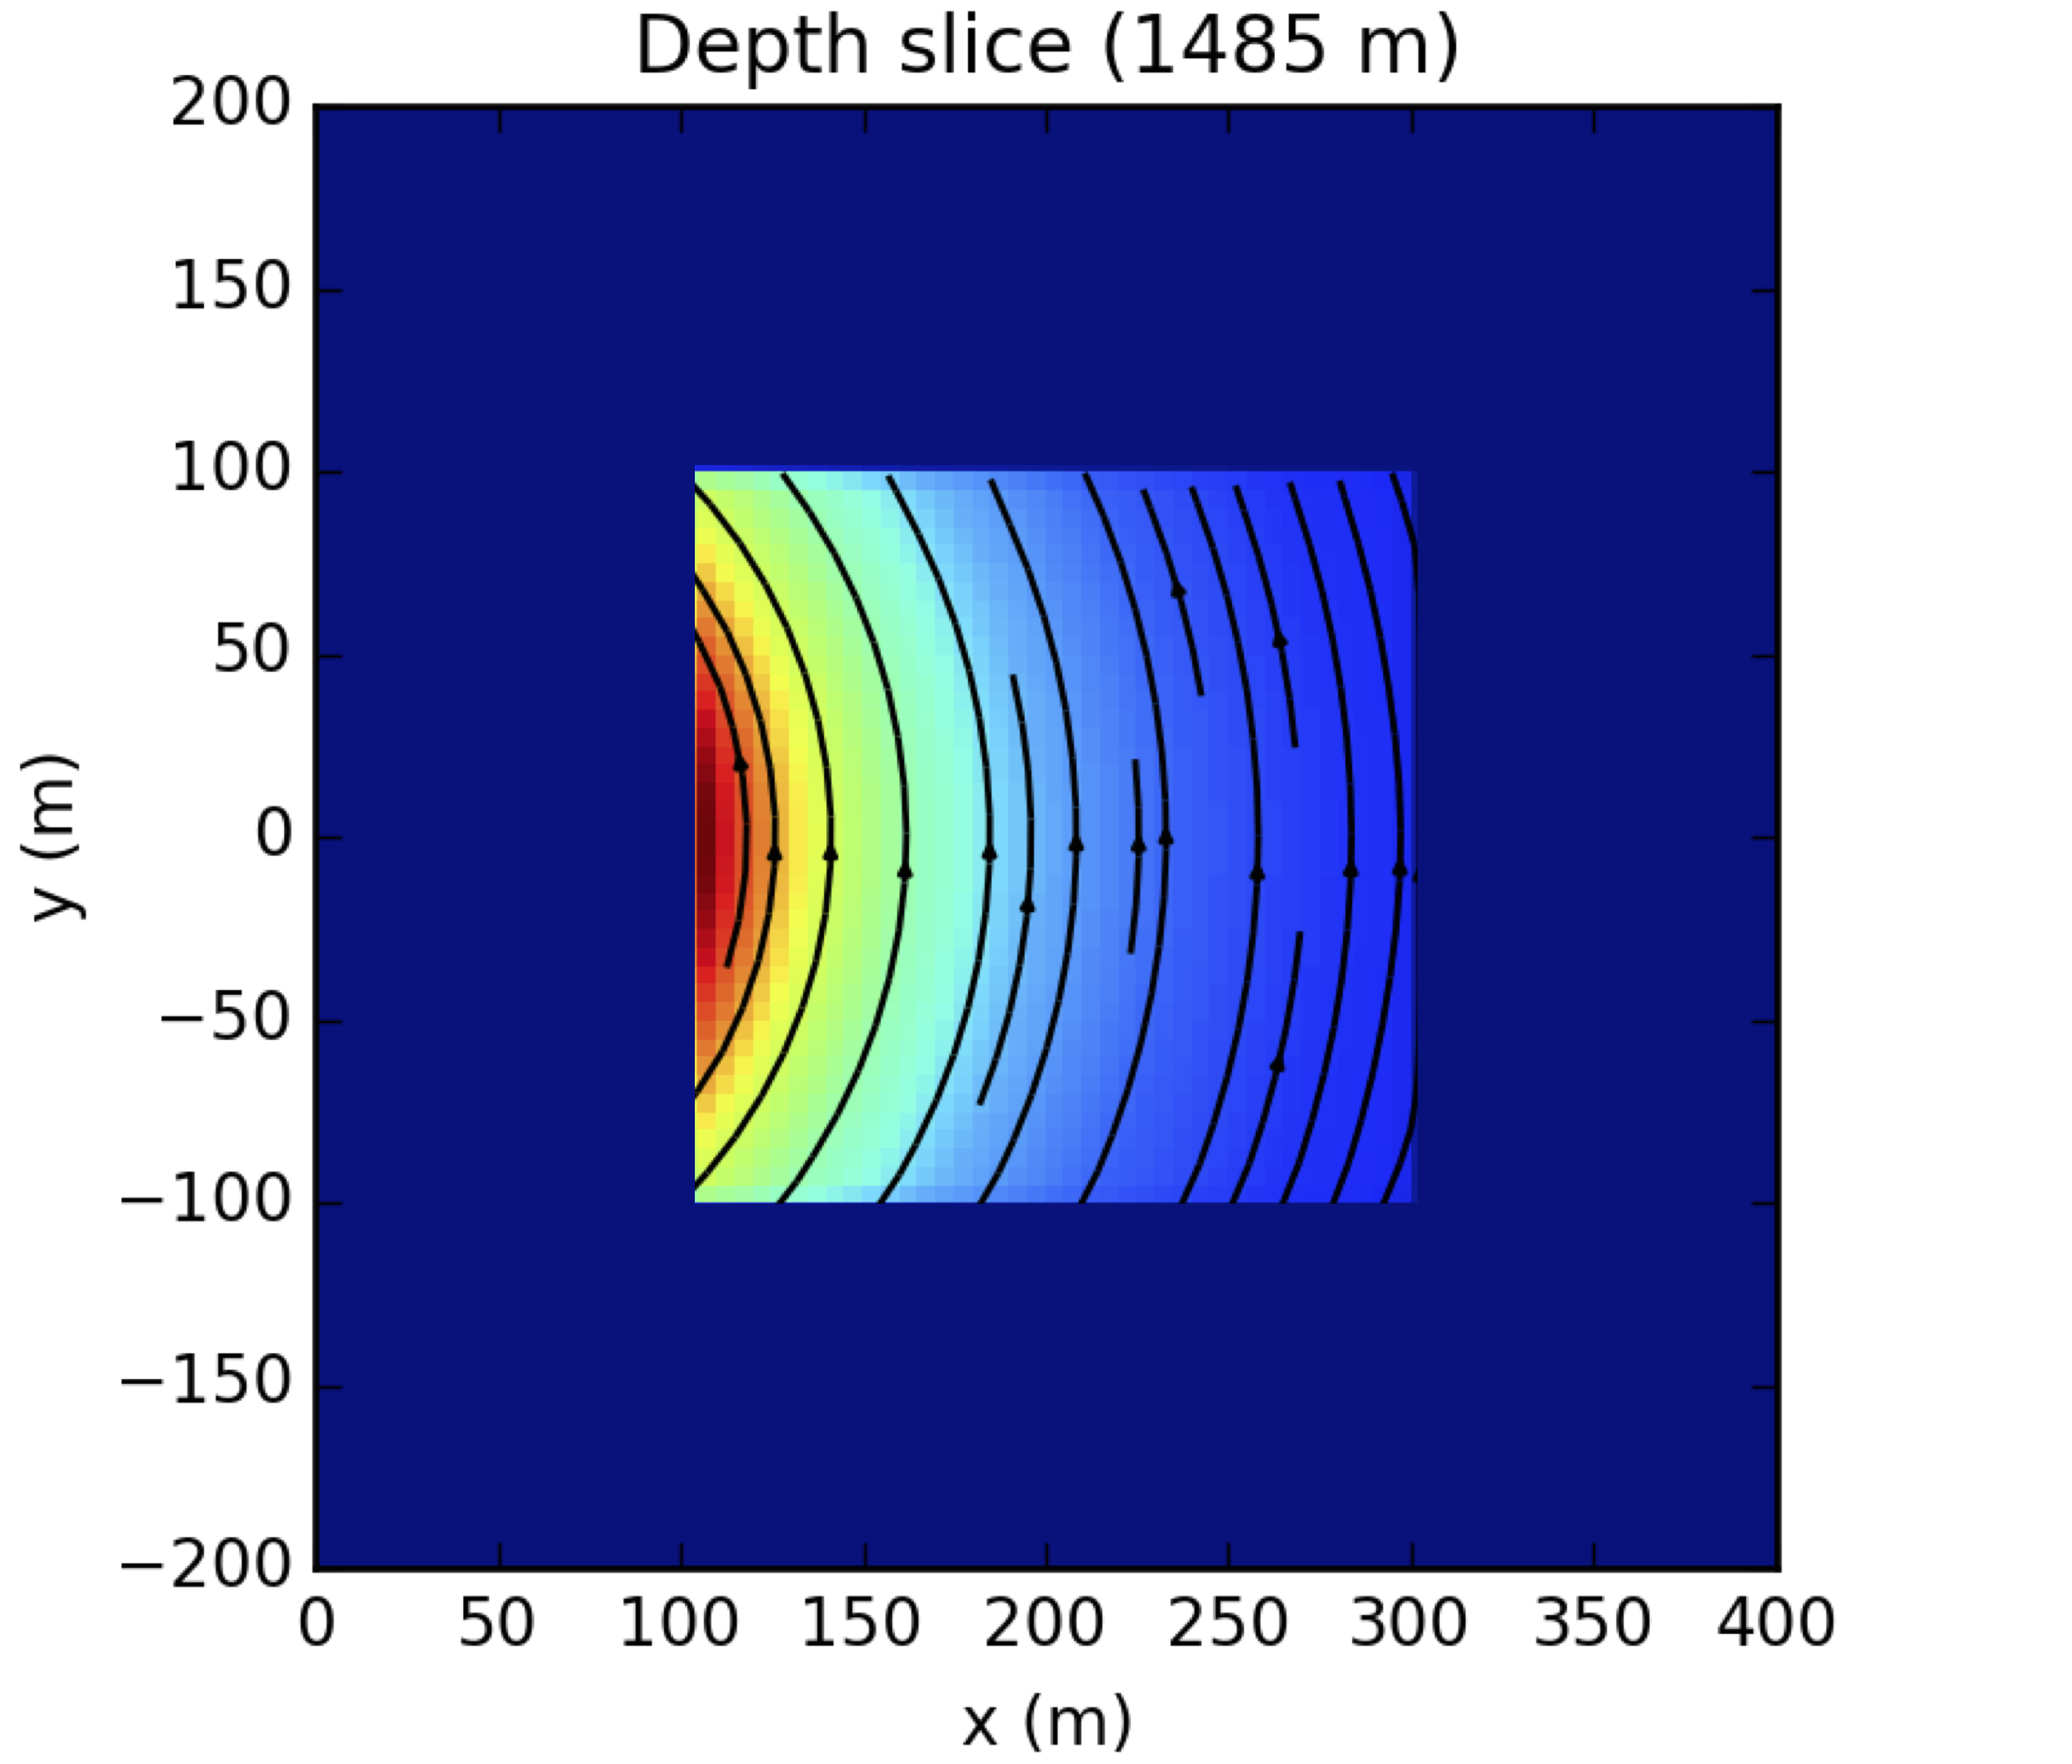
\includegraphics[width=0.95\columnwidth]{./Figures/SecSource}
	\caption{Depth slice of the source for the secondary problem. }
	\label{fig:secondarySource}
\end{figure}
With the source term for the secondary problem defined, the associated fields and fluxes can then be simulated. The data are then a projection of the sum of the primary and secondary responses to the receiver locations.

\subsection{Inversion}
The primary-secondary approach is well-suited for tackling the inverse problem in this setting. The primary, consisting of the well and a simple geologic model (which may be derived from well logs) can be computed once and used directly as the source for computing the secondary problem, requiring no extra processing on the measured data. The computed primary fields are interpolated to the mesh which we use for computing the secondary responses, and the inversion can be carried out by computing forward problems on this mesh alone. Note that the right hand side of equation \ref{eq:secondary} depends on the physical property model and needs to be accounted for in the sensitivities when doing gradient-based optimization.

Such an approach provides opportunity for a significant reduction in the computational load required by a more traditional approach to the inverse problem where the full forward model, including the casing, must be considered at every iteration. Additionally, no intermediate inversion or analysis, for constructing an  ``equivalent source'', composed of point sources or dipoles is required. For the example we demonstrated, the casing, background geologic model and source location supported the use of a cylindrical mesh for the computation of the primary. In general, the background geology, well path, and source location may not adhere to this symmetry requiring a different strategy for computing the primary. This will likely require an expensive computation on a mesh which has been highly refined near the wellbore. Using the primary-secondary approach, however, means that only one such computation is required to address the inverse problem.

% \vspace{-8pt}
\section{Conclusion}
% \vspace{-8pt}
Using the primary-secondary approach for modelling EM surveys in settings where cased wells are present allows for a separation of concerns between accurately modelling well casing and modelling three dimensional geologic structures. In the first step, the source and casing are modelled in a simple geologic background.
Well casing has significant electrical conductivity and magnetic permeability, both of which may be variable along the length of the well. This makes the casing a complicated structure to model, but an important one, as the large contrasts in physical properties it presents means that it may have a significant impact on the EM fields and fluxes.
Much investigation remains to better understand how each of the complexities introduced by the casing impacts the behavior of the EM signals being used to excite responses in the surrounding geologic units. In the second step, the computed primary fields are used as a source for the secondary problem: simulating the behavior of the EM fields and fluxes in the presence of three dimensional geologic structures. This procedure removes concerns of accurately simulating the casing at this step, as the interaction of the source with the casing is captured in the computation of the primary response, and contained in the definition of the source for the secondary problem. When considering the inverse problem, this separation of concerns provides the benefit that the computation of the casing response need only be completed once. The remainder of the inversion is completed on a mesh suitable for characterizing the variations in the geologic structures of interest.

% \vspace{-10pt}
\section{Acknowledgements}
% \vspace{-10pt}
The authors thank the contributors to \href{http://simpeg.xyz}{\SimPEG}  and \href{https://github.com/simpeg/simpegem}{\simpegEM}, in particular: Seogi Kang and Adam Pidlisecky. We also thank Eldad Haber and Christoph Schwarzbach.
% for their insightful comments on the numerical implementation. Funding for this work was provided through NSERC.

\onecolumn


\bibliographystyle{seg}  % style file is seg.bst
\bibliography{bibliography.bib}

\end{document}
